\documentclass[12pt, oneside]{article}   	% use "amsart" instead of "article" for AMSLaTeX format

%%%%%%%%%%%%%%%%%%%%%%%%%%%%%%%%%%%%%%%%%%%%%%%%%%%%
% set up packages, geometry
%%%%%%%%%%%%%%%%%%%%%%%%%%%%%%%%%%%%%%%%%%%%%%%%%%%%
\usepackage{geometry, textcomp, amsmath, graphicx, amssymb,fancyhdr,subcaption,bm}                
	
\geometry{letterpaper, marginparwidth=60pt}                   		
\usepackage[superscript,noadjust]{cite} % puts dash in citations to abbreviate
%\usepackage [autostyle, english = american]{csquotes} % sets US-style quotes
%\MakeOuterQuote{"} % sets quote style

\usepackage{geometry}                
\usepackage{textcomp}                
\usepackage{amsmath}                
\usepackage{graphicx}                
\usepackage{amssymb}                
\usepackage{fancyhdr}                
\usepackage{subcaption}                
\usepackage{bm}                
\usepackage{lineno}
\usepackage{pdfpages}
\usepackage{etoolbox}

\AtBeginEnvironment{quote}{\small}

\usepackage{float,color}

\usepackage{pgf, tikz, eqnarray}

\usetikzlibrary{fit}
\usetikzlibrary{positioning}


\usetikzlibrary{arrows, automata}
%%%%%%%%%%%%%%%%%%%%%%%%%%%%%%%%%%%%%%%%%%%%%%%%%%%%

%%%%%%%%%%%%%%%%%%%%%%%%%%%%%%%%%%%%%%%%%%%%%%%%%%%%
\pagestyle{plain}                                                      %%
%%%%%%%%%% EXAFT 1in MARGINS %%%%%%%                                   %%
\setlength{\textwidth}{6.5in}     %%                                   %%
\setlength{\oddsidemargin}{0in}   %% (It is recommended that you       %%
\setlength{\evensidemargin}{0in}  %%  not change these parameters,     %%
\setlength{\textheight}{8.5in}    %%  at the risk of having your       %%
\setlength{\topmargin}{0in}       %%  proposal dismissed on the basis  %%
\setlength{\headheight}{0in}      %%  of incorrect formatting!!!)      %%
\setlength{\headsep}{0in}         %%                                   %%
\setlength{\footskip}{.5in}       %%                                   %%
%%%%%%%%%%%%%%%%%%%%%%%%%%%%%%%%%%%%                                   %%		

%%%%%%%%%%%%%
% DEFINE CODE BLOCK
%%%%%%%%%%%%%
\usepackage{listings}

\definecolor{dkgreen}{rgb}{0,0.6,0}
\definecolor{gray}{rgb}{0.5,0.5,0.5}
\definecolor{mauve}{rgb}{0.58,0,0.82}

\lstset{frame=tb,
  language=R,
  aboveskip=3mm,
  belowskip=3mm,
  showstringspaces=false,
  columns=flexible,
  basicstyle={\small\ttfamily},
  numbers=none,
  numberstyle=\tiny\color{gray},
 % keywordstyle=\color{blue},
  commentstyle=\color{dkgreen},
  stringstyle=\color{mauve},
  breaklines=true,
  breakatwhitespace=true,
  tabsize=3,
  otherkeywords={0,1,2,3,4,5,6,7,8,9},
  deletekeywords={data,frame,length,as,character,dunif,ps},
}

\begin{document}

\section*{Appendix X}

There are two ways that we can calculate transition probabilities in the seed bank with data from seed burial experiments and viability tests. Both take into account the fact that outcomes in these experiments are conditional on previous outcomes. For example, seeds that germinate in the first January must first have remained intact and viable. 

One approach to this problem is to change the denominator for all of our calculations. In this case, the rate is calculated based on the subset of possible seeds. For example, the number of seeds that survive to January is the sum of seeds that germinate and seeds that are estimated to be viable. This value is the numerator in calculating $s_1$, and then becomes the denominator in calculating $g_1$. This method states that the number of seeds that are viable is known with the same amount of certainty as the number of seeds that germinate. In fact, our estimate of viability in January probably has a greater amount of uncertainty. 

A second approach to this problem is to include uncertainty about estimates in all of the calculations. We can do this by calculating the transition probabilities as conditional probabilities. 

Below, I calculate each transition probability using both methods. The figure below shows the results of a simulation study indicating that the two approaches are directly comparable. 
%
 \begin{figure}[h]
   \centering
  %#\begin{tabular}{@{}c@{\hspace{.5cm}}c@{}}
       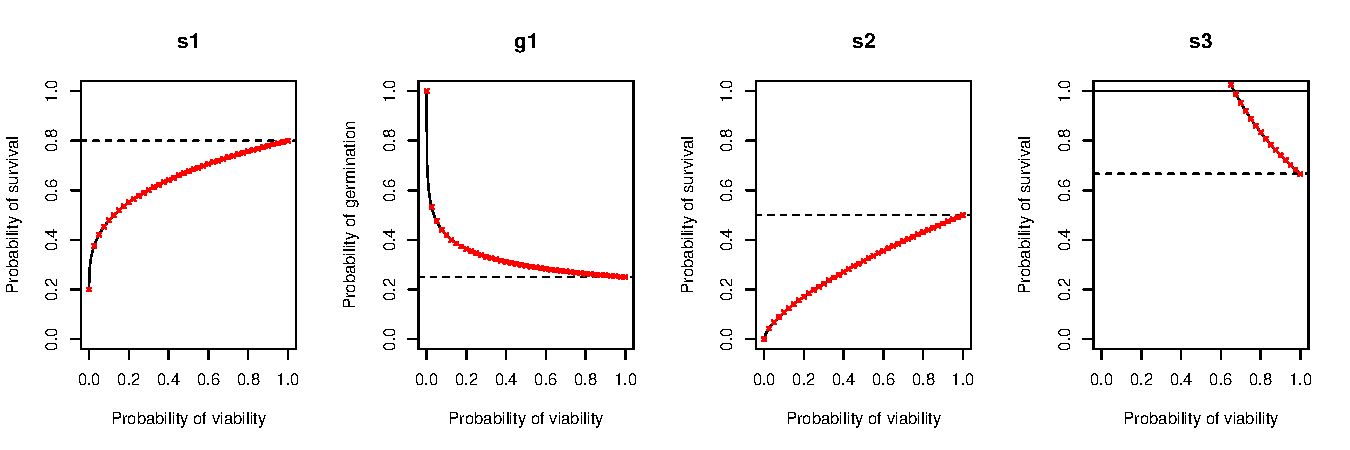
\includegraphics[page=1,width=\textwidth]{../figures/appendix/comparison}  
    \caption{ (A) This plot compares estimated probabilities for the following values (total = 100, yjan = 60, ygerm = 20, yoct = 50) for a range of possible viability. The line is the changing denominator approach, the red crosses are the conditional probability approach. The estimate for s3 is for $\nu_2 = 1$. }
 \label{fig:comparison}
\end{figure}
%
\subsection*{s1}

We define $s_1$ as the probability of a seed being intact and viable from October in year $t$ to January in year $t+1$. We want this estimate to include seeds that germinated and seeds that were intact and viable. To obtain this estimate, we have data on the following quantities:

\begin{itemize}
	\item $n^{total}$ = the number of seeds that started the seed bag experiments
	\item $y^{germ}$ = the number of seedlings in January
	\item $y^{jan1}$ = the number of intact seeds in January of year $t+1$
	\item $\nu$ = the probability that a seed that is intact in October of year $t+1$ is viable (estimated elsewhere)
\end{itemize}

We can use this information to calculate the $s_1$ in two ways. First, we can estimate the fraction of seeds that are intact and viable in January as $y^{jan1}\times \nu^{1/3}$. We then calculate 
%
    \begin{align}
\begin{split}
s_1 = \frac{y^{jan1}\times \nu^{1/3} + y^{germ}}{n^{total}}
  \end{split}
\end{align}
%
Alternatively, we can compose an estimate for $s_1$ using two conditional probabilities. First, we estimate the probability of a seed being intact to January as $p^{intact} = (y^{germ}+y^{jan1})/n^{total}$. Second, we estimate the probability of a plant emerging, conditional on being intact as $p^{germ} = y^{germ}/(y^{germ}+y^{jan1})$. We then calculate 
%
    \begin{align}
\begin{split}
s_1 = p^{intact} \times (p^{germ} + ( 1- p^{germ} ) \times \nu^{1/3} )
  \end{split}
\end{align}
%

\subsection*{g1}

We define $g_1$ as the probability of germination for a seed that is intact and viable. To obtain this estimate, we have data on the following quantities:

\begin{itemize}
	\item $n^{total}$ = the number of seeds that started the seed bag experiments
	\item $y^{germ}$ = the number of seedlings in January
	\item $y^{jan1}$ = the number of intact seeds in January of year $t+1$
	\item $\nu$ = the probability that a seed that is intact in October of year $t+1$ is viable (estimated elsewhere)
\end{itemize}

We can use this information to calculate the $g_1$ in two ways. First, we can estimate the fraction of seeds that are intact and viable in January as $y^{jan1}\times \nu^{1/3}$. We then calculate 
%
    \begin{align}
\begin{split}
g_1 = \frac{ y^{germ}}{y^{jan1}\times \nu^{1/3} + y^{germ}}
  \end{split}
\end{align}
%
Alternatively, we can compose an estimate for $g_1$ using conditional probabilities. First, we estimate the probability of a plant emerging, conditional on being intact as $p^{germ} = y^{germ}/(y^{germ}+y^{jan1})$. We then calculate 
%
    \begin{align}
\begin{split}
g_1 = \frac{p^{germ} }{1 - ( 1-  \nu^{1/3} ) \times ( 1 - p^{germ} )}
  \end{split}
\end{align}
%

\subsection*{s2}

We define $s_2$ as the probability of survival from January to October in year $t$ for a seed that was intact and viable in January. To obtain this estimate, we have data on the following quantities:

\begin{itemize}
	\item $n^{total}$ = the number of seeds that started the seed bag experiments
	\item $y^{germ}$ = the number of seedlings in January
	\item $y^{jan1}$ = the number of intact seeds in January of year $t+1$
	\item $y^{oct1}$ = the number of intact seeds in January of year $t+1$
	\item $\nu$ = the probability that a seed that is intact in October of year $t+1$ is viable (estimated elsewhere)
\end{itemize}

We can use this information to calculate the $s_2$ in two ways. First, we can estimate the fraction of seeds that are intact and viable in January as $y^{jan1}\times \nu^{1/3}$. Second, we can estimate the fraction of seeds that are intact and viable in October as $y^{oct1}\times \nu$ We then calculate 
%
    \begin{align}
\begin{split}
s_2 = \frac{ y^{oct1}\times \nu }{ y^{jan1}\times \nu^{1/3} }
  \end{split}
\end{align}
%
Alternatively, we can compose an estimate for $s_2$ using conditional probabilities. First, we estimate the probability of a seed being intact in October, conditional on being intact in January $ p = y^{oct1} / y^{jan1} $. We then calculate 
%
    \begin{align}
\begin{split}
s_2 = p \times \nu^{2/3}
  \end{split}
\end{align}
%
\subsection*{s3}

We define $s_3$ as the probability of survival from October in year $t$ to January in year $t+1$ for a seed that was intact and viable in October. To obtain this estimate, we have data on the following quantities:

\begin{itemize}
	\item $n^{total}$ = the number of seeds that started the seed bag experiments
	\item $y^{germ}$ = the number of seedlings in January
	\item $y^{jan1}$ = the number of intact seeds in January of year $t+1$
	\item $y^{oct1}$ = the number of intact seeds in January of year $t+1$
	\item $y^{germ2}$ = the number of seedlings in January year 2
	\item $y^{jan2}$ = the number of intact seeds in January of year 2
	\item $\nu$ = the probability that a seed that is intact in October of year $t+1$ is viable (estimated elsewhere)
	\item $\nu_2$ = the probability that a seed that is intact in October of year $t+2$ is viable (estimated elsewhere)

\end{itemize}

We can use this information to calculate the $s_3$ in two ways. First, we can estimate the fraction of seeds that are intact and viable in October as $y^{oct1}\times \nu$. Second, we can estimate the fraction of seeds that are intact and viable in January as $y^{jan2}\times \nu_2^{1/3}$. We then calculate 
%
    \begin{align}
\begin{split}
s_3 = \frac{y^{jan2}\times \nu_2^{1/3} + y^{germ2}}{y^{oct1}\times \nu}
  \end{split}
\end{align}
%
Alternatively, we can compose an estimate for $s_3$ using conditional probabilities. First, we make use the probabilities for $s_1$, $g_1$ and $s_2$ (described above) to normalize the event space. Second, we estimate the probability of a seed being intact to January as $p^{intact} = (y^{germ2}+y^{jan2})/n^{total}$. Finally, we estimate the probability of a plant emerging, conditional on being intact as $p^{germ2} = y^{germ2}/(y^{germ2}+y^{jan2})$. We then calculate 
%
    \begin{align}
\begin{split}
s_3 = \frac{p^{intact} \times (p^{germ2} + ( 1- p^{germ2} ) \times \nu_2^{1/3} )}{s_1 \times (1-g_1) \times s_2 }
  \end{split}
\end{align}
%

\subsection*{Adjusting viability in year 2}

For the 2011 paper, the following was applied. If viability estimated in the second year was less than viability estimated in the first year, the probability of viability in January of year 2 was interpolated as $\nu^{2/3} \times \nu_2^{1/3} $. If viability estimated in the second year was equal to or greater than viability estimated in the first year, the probability of viability in January of year 2 was estimated as $\nu_2^{1/3} $. 

By calculating viability using the approach described in this appendix, I did not encounter a situation where the estimate was greater than one.  I thus always calculated the probability of viability in January of year 2 was interpolated as $\nu^{2/3} \times \nu_2^{1/3} $.

\iffalse

\subsection*{Conditional probabilities}
This appendix shows that the probability of germination, conditional on seeds being viable and intact, can be calculated from the probability of viability conditional on being intact and not germinating $v^{1/3}$ and the probability of being a seedling conditional on being intact, $\theta^g$. In the model fitting process, we estimate the probabilities on the right hand side of the equation below, and use that to derive the probability of germination, conditional on seeds being viable and intact.

    \begin{align}
\begin{split}
P(G | V \cap I)  = g_1 = \frac{n^{\mathrm{germinants}}}{n^{\mathrm{intact}}\times v^{1/3} + n^{\mathrm{germinants}}} = \frac{ \theta^g }{ 1-(1-\theta^v)(1-\theta^g)}
  \end{split}
\end{align}

The plot below shows that the two methods produce the same estimates for the probability of germination, a given number of intact seeds and number of seeds that are germinated.  

\subsection*{Conditional probability tree}

Here's a conditional probability tree to graphically represent the events in the seed bag experiments. The seed bags are buried, some are intact and/or germinate ($I$), some are viable ($V$), and some germinate ($G$). 

 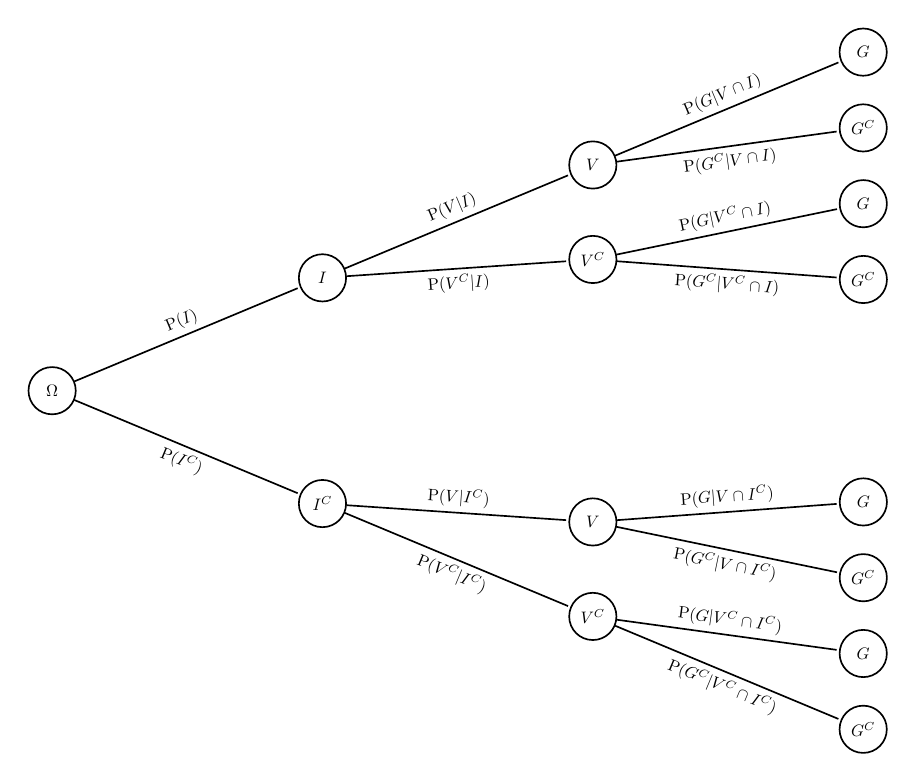
\begin{tikzpicture}[
            > = stealth, % arrow head style
            shorten > = 1pt, % don't touch arrow head to node
            auto,
            node distance = 2cm, % distance between nodes
            semithick, % line style
            scale=0.6, every node/.style={scale=0.6}
        ]

        \tikzstyle{every state}=[
            draw = none,
            thick,
            fill = white,
            minimum size = 4mm
        ]F

       \node[circle,draw,minimum size = 1cm] (T) {$\Omega $};
     
       \node[circle,draw,minimum size = 1cm] (I) [above right=1cm and 3cm of T] {$I$};
	\node[circle,draw,minimum size = 1cm] (IC) [below right=1cm and 3cm of T] {$I^C$};

        \node[circle,draw,minimum size = 1cm] (IV) [above right=1cm and 3cm of I] {$V$};
	\node[circle,draw,minimum size = 1cm] (IVC) [below of=IV] {$V^C$};
	
	\node[circle,draw,minimum size = 1cm] (IVG) [above right=1cm and 3cm of IV] {$G$};
	\node[circle,draw,minimum size = 1cm] (IVGC) [below = .35cm of IVG] {$G^C$};
	\node[circle,draw,minimum size = 1cm] (IVCG) [below = .35cm of IVGC] {$G$};
	\node[circle,draw,minimum size = 1cm] (IVCGC) [below = .35cm of IVCG] {$G^C$};

	\node[circle,draw,minimum size = 1cm] (ICVC) [below right=1cm and 3cm of IC] {$V^C$};
        \node[circle,draw,minimum size = 1cm] (ICV) [above of=ICVC] {$V$};

	\node[circle,draw,minimum size = 1cm] (ICVCGC) [below right = 1cm and 3 cm of ICVC] {$G^C$};
	\node[circle,draw,minimum size = 1cm] (ICVCG) [above = .35cm of  ICVCGC] {$G$};
	\node[circle,draw,minimum size = 1cm] (ICVGC) [above = .35cm of ICVCG] {$G^C$};        
        	\node[circle,draw,minimum size = 1cm] (ICVG) [above = .35cm of ICVGC] {$G$};

	\path[-]	
            (T)    edge  node[sloped, anchor=center, above] {P($I$)}     (I)
            (T)    edge  node[sloped, anchor=center, below] {P($I^C$)}          (IC)
            (I)    edge  node[sloped, anchor=center, above] {P($V|I$)} (IV)
            (I)    edge  node[sloped, anchor=center, below] {P($V^C|I$)}         (IVC)
            (IC)    edge  node[sloped, anchor=center, above] {P($V|I^C$)} (ICV)
            (IC)    edge  node[sloped, anchor=center, below] {P($V^C|I^C$)}         (ICVC)
                     
            (IV)    edge  node[sloped, anchor=center, above] {P($G|V \cap I$)} (IVG)
            (IV)    edge  node[sloped, anchor=center, below] {P($G^C|V \cap I$)}         (IVGC)
            
            (IVC)    edge  node[sloped, anchor=center, above] {P($G|V^C \cap I$)} (IVCG)
            (IVC)    edge  node[sloped, anchor=center, below] {P($G^C|V^C \cap I$)}         (IVCGC)
            
            (ICV)    edge  node[sloped, anchor=center, above] {P($G|V \cap I^C$)} (ICVG)
            (ICV)    edge  node[sloped, anchor=center, below] {P($G^C|V \cap I^C$)}         (ICVGC)
            
            (ICVC)    edge  node[sloped, anchor=center, above] {P($G|V^C \cap I^C$)} (ICVCG)
            (ICVC)    edge  node[sloped, anchor=center, below] {P($G^C|V^C \cap I^C$)}         (ICVCGC);

        
  \end{tikzpicture} \newline

  
  
 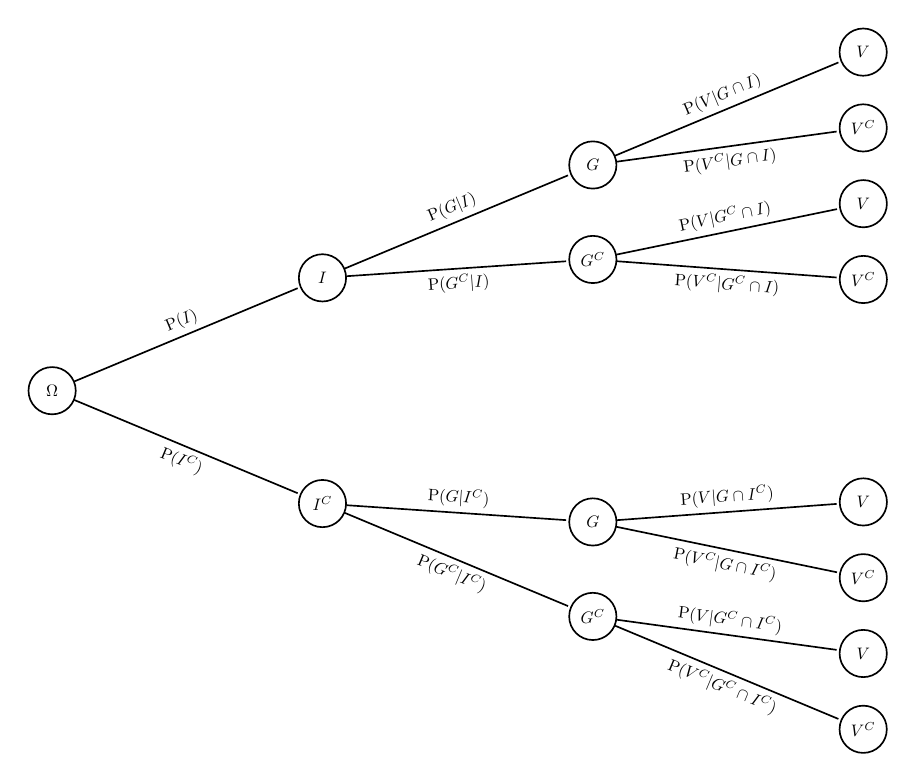
\begin{tikzpicture}[
            > = stealth, % arrow head style
            shorten > = 1pt, % don't touch arrow head to node
            auto,
            node distance = 2cm, % distance between nodes
            semithick,
            scale=0.6, every node/.style={scale=0.6} % line style
        ]

        \tikzstyle{every state}=[
            draw = none,
            thick,
            fill = white,
            minimum size = 4mm
        ]F

       \node[circle,draw,minimum size = 1cm] (T) {$\Omega $};
     
       \node[circle,draw,minimum size = 1cm] (I) [above right=1cm and 3cm of T] {$I$};
	\node[circle,draw,minimum size = 1cm] (IC) [below right=1cm and 3cm of T] {$I^C$};

        \node[circle,draw,minimum size = 1cm] (IG) [above right=1cm and 3cm of I] {$G$};
	\node[circle,draw,minimum size = 1cm] (IGC) [below of=IG] {$G^C$};
	
	\node[circle,draw,minimum size = 1cm] (IGV) [above right=1cm and 3cm of IG] {$V$};
	\node[circle,draw,minimum size = 1cm] (IGVC) [below = .35cm of IGV] {$V^C$};
	\node[circle,draw,minimum size = 1cm] (IGCV) [below = .35cm of IGVC] {$V$};
	\node[circle,draw,minimum size = 1cm] (IGCVC) [below = .35cm of IGCV] {$V^C$};

	\node[circle,draw,minimum size = 1cm] (ICGC) [below right=1cm and 3cm of IC] {$G^C$};
        \node[circle,draw,minimum size = 1cm] (ICG) [above of=ICGC] {$G$};

	\node[circle,draw,minimum size = 1cm] (ICGCVC) [below right = 1cm and 3 cm of ICGC] {$V^C$};
	\node[circle,draw,minimum size = 1cm] (ICGCV) [above = .35cm of  ICGCVC] {$V$};
	\node[circle,draw,minimum size = 1cm] (ICGVC) [above = .35cm of ICGCV] {$V^C$};        
        	\node[circle,draw,minimum size = 1cm] (ICGV) [above = .35cm of ICGVC] {$V$};

	\path[-]	
            (T)    edge  node[sloped, anchor=center, above] {P($I$)}     (I)
            (T)    edge  node[sloped, anchor=center, below] {P($I^C$)}          (IC)
            (I)    edge  node[sloped, anchor=center, above] {P($G|I$)} (IG)
            (I)    edge  node[sloped, anchor=center, below] {P($G^C|I$)}         (IGC)
            (IC)    edge  node[sloped, anchor=center, above] {P($G|I^C$)} (ICG)
            (IC)    edge  node[sloped, anchor=center, below] {P($G^C|I^C$)}         (ICGC)
                     
            (IG)    edge  node[sloped, anchor=center, above] {P($V|G \cap I$)} (IGV)
            (IG)    edge  node[sloped, anchor=center, below] {P($V^C|G \cap I$)}         (IGVC)
            
            (IGC)    edge  node[sloped, anchor=center, above] {P($V|G^C \cap I$)} (IGCV)
            (IGC)    edge  node[sloped, anchor=center, below] {P($V^C|G^C \cap I$)}         (IGCVC)
            
            (ICG)    edge  node[sloped, anchor=center, above] {P($V|G \cap I^C$)} (ICGV)
            (ICG)    edge  node[sloped, anchor=center, below] {P($V^C|G \cap I^C$)}         (ICGVC)
            
            (ICGC)    edge  node[sloped, anchor=center, above] {P($V|G^C \cap I^C$)} (ICGCV)
            (ICGC)    edge  node[sloped, anchor=center, below] {P($V^C|G^C \cap I^C$)}         (ICGCVC);

        
  \end{tikzpicture} \newline
  

  We have these estimates
  
  \begin{itemize}
	\item P($I$) = in January, the seeds that are intact and germinated
	\item P($G|I$) = in January, the seeds that germinated given that they were intact 
	\item P($V|G \cap I$) = in January, the seeds that were viable given that they germinated and were intact (we assume this is $1$; all seeds that germinate are viable)
	\item P($G^C|V^C \cap I$) = in January, the seeds that were intact but not viable did not germinate (we assume this is $1$; any seed that is not viable can not germinate)
		\item P($V|G^C \cap I$) = in January, the seeds that viable given that they are intact and that not germinate (this is $v^{\frac{1}{3}}$)
\end{itemize}
  
The germination probability, $g_1$, is the probability that seeds germinate given that they are intact and viable. Put another way: of the viable seeds, how many germinate? In our probability tree, this is $g_1 = P(G | V \cap I)$. The conditional probability trees give the following equalities:
  
  \begin{align}
\begin{split}
	P(V \cap G \cap I) &= P(V | G \cap I) P(G | I) P(I) \\
	P(G \cap V \cap I) &= P(G | V \cap I) P(V | I) P(I) \label{eq:fullConditional}	
  \end{split}
\end{align}

To solve for this, we start by solving for P($V|I$). More accurately, we solve for P($V^C|I$) and use this to get P($V|I$) = 1-P($V^C|I$).

  \begin{align}
\begin{split}
	P(V^C \cap G^C \cap I) &= P(G^C \cap V^C \cap I) \\
	P(V^C | G^C \cap I) P(G^C | I) P(I) &= P(G^C | V^C \cap I) P(V^C | I) P(I) 	\\
	P(V^C | I) &= \frac{ P(V^C | G^C \cap I) P(G^C | I) P(I) }{P(G^C | V^C \cap I) P(I)}\\
  \end{split}
\end{align}

We can then cancel out the probability of being intact. We also use P($V^C | G^C \cap I$) = 1-P($V | G^C \cap I$), P($G^C | I$) = 1-P($G | I$) and the assumption that P($G^C|V^C \cap I$) = 1 to rewrite the expression:

  \begin{align}
\begin{split}
	P(V^C | I) &=  ( 1-P(V | G^C \cap I) ) (1 - P(G | I)  )
  \end{split}
\end{align}

We then substitute the probability of viability for seeds that are intact but did not germinate, P($V | G^C \cap I$), and the probability of germination for seeds that are intact, P($G|I$). We solve for P($V | I$) = 1-P($V^C | I$) 

  \begin{align}
\begin{split}
	P(V | I) &= 1-  ( 1-P(V | G^C \cap I) ) (1 - P(G | I)  )
  \end{split}
\end{align}

We can set these expressions in equation~\eqref{eq:fullConditional} equal to each other, which allows us to solve for  $g_1 = P(G | V \cap I)$:

  \begin{align}
\begin{split}
	P(V \cap G \cap I) &= P(G \cap V \cap I) \\
	P(G | V \cap I) P(V | I) P(I) &= P(V | G \cap I) P(G | I) P(I) \\
	P(G | V \cap I)  &= \frac{P(V | G \cap I) P(G | I)  P(I)}{P(V | I)  P(I) } \\
	P(G | V \cap I)  &= \frac{ P(G | I)  P(I)}{P(V | I)  P(I) }
  \end{split}
\end{align}
  
We use P($V|G \cap I$) = 1. We are then left with a statement saying that the probability of germination for seeds that are viable and intact is the probability of germination, conditional on being intact, divided by the probability of being viable, conditional on being intact. The probabilities of being intact cancel and we can use our solution for the probability of being viable conditional on being intact as well as the independently  
 
    \begin{align}
\begin{split}
	P(G | V \cap I)  &= \frac{ P(G | I)  P(I)}{P(V | I)  P(I) }
  \end{split}
\end{align}

We use this relationship to calculate the probability of germination conditional on being viable and intact as a derived quantity of estimates for the probability of germination conditional on being intact, and of the probability of being viable conditional on being intact. 

    \begin{align}
\begin{split}
	P(G | V \cap I)  &= \frac{ \theta^g }{ 1-(1-\theta^v)(1-\theta^g)}
  \end{split}
\end{align}

Where $\theta^g$ is the probability of a bag having germinants and $\theta^v$ is the probability of viability in January.  
\fi

\end{document}